
\chapter{SYSTEM IMPLEMENTATION }
\thispagestyle{empty}
\\

\par The implementation is divided into five parts.
\begin{enumerate}
    \item Data Pre-processing
    \item Feature Extraction
    \item Model Comparison
    \item Model Evaluation
    \item Model Implementation
\end{enumerate}

\section{DATA PRE-PROCESSING}
\par Data pre-processing is an essential step in preparing raw data for analysis and machine learning tasks. It involves transforming and cleaning the data to ensure its quality, consistency, and suitability for further analysis.
We obtained two separate datasets from different sources and merged them to create a larger dataset for training and testing our machine learning models.
\subsubsection{Data Cleaning}
\par In the Dataset-I (url and label as columns), we found 92 urls without any corresponding label values i.e, having null values. and these rows were dropped from this datasets.
\subsubsection{Data Reduction}
We only need the urls and there corresponding label values(1 0r 2 representing phishing or legitimate) as the input datas, the Dataset-II contains unwanted columns so they are also dropped.
\subsubsection{Data Integration}
Next we will be merging our 2 datasets , for that we will be considering the Datatypes and names of the columns to avoid damage of the resultant dataset after merging. Merging DataFrames with different data types for the same column name might lead to inconsistencies and unexpected behavior and merging DataFrames having different column names produce splitting of the values. So they both are handled before merging. After Merging we obtained a dataset having 546,104 datas and saved in a new csv file.

\par After merging there are chances of having duplicate data inside the resultant dataset. There were 194 Duplicate URLs in our resultant dataset. And these were dropped. Fig 4.2 shows the 
Bar-Graph Classification of Phishing and Legitimate urls inside the new dataset:

\begin{figure}[H] 
  \centering
  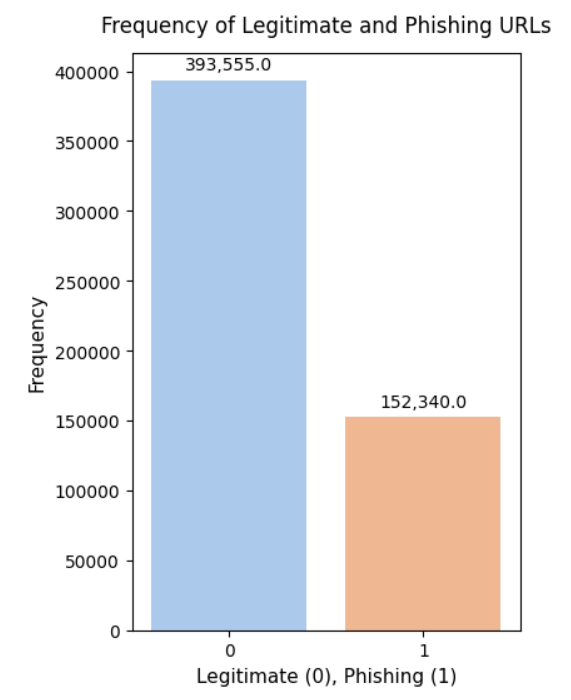
\includegraphics[scale=0.6]{barGraph_PorL.png} 
  \caption{Bar-Graph Classification of Phishing and Legitimate data.}
  \label{fig}
\end{figure}

\begin{figure}[H] 
  \centering
  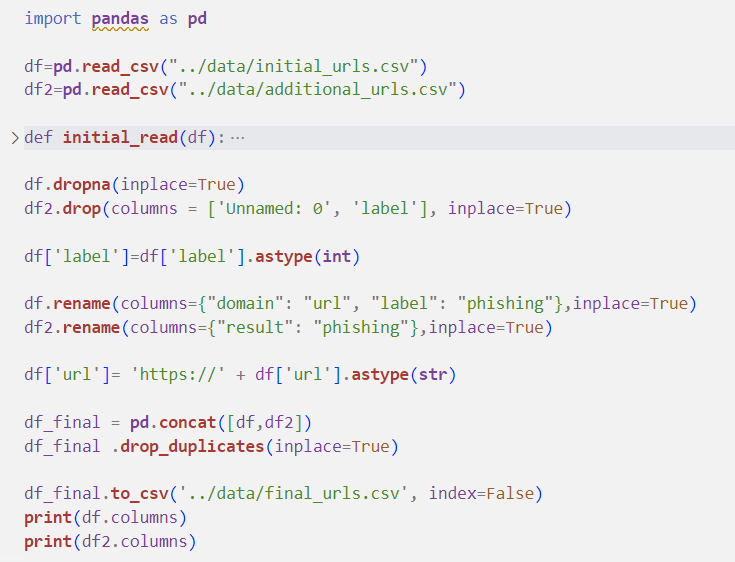
\includegraphics[scale=0.68]{DataPreprocessing_Code.png} 
  \caption{Data Pre-Processing}
  \label{fig}
\end{figure}

\section{FEATURE EXTRACTION}
\par Feature extraction is a technique used to reduce the dimensionality of data by transforming the raw input into a set of derived features that capture the essential information. It aims to highlight the most relevant aspects of the data and discard irrelevant or redundant information. 
\par In our project, the features are generally classified into two:
\begin{enumerate}
  \item Lexical Features
  \item Numerical Features
\end{enumerate}
\subsection{Lexical Features}
\par Lexical features in URL feature extraction involve analyzing the textual components and patterns within a URL. These features capture characteristics related to the structure, keywords, symbols, and other textual elements of a URL.
\begin{itemize}
  \item getEntropy :-{ It is known that DGA(Domain Generation Algorithm) domains have a greater level of disorderliness in their alphabetic distribution. Legitimate domains tend to have well-defined names that speak to a brand or a product so tend to be less disorganized. Thus, measuring the entropy of URL strings tells us which domain names are ‘not-so-real.}
  \item hasLogin :-{Check if the URL contains specific keyword "login," .We can capture the fact that certain ‘red flag’ keywords appear in a URL string. These keywords may relate to keywords attackers use when trying to spoof a legitimate page or keywords that relate to popular nomenclature of security settings on a website that a hacker will try to manipulate.So,If the URL string contains “login” keyword, the value assigned to this feature is 1 (phishing) or else 0 (legitimate).}
  \item Redirection :-{ Phishing attackers often employ redirection techniques to hide the true destination of a malicious URL. By redirecting users through multiple URLs or using URL shorteners, they can make it more difficult for users and security systems to identify the final destination. Checks the presence of "//" in the URL. The existence of “//” within the URL path means that the user will be redirected to another website.(avoiding the "//" after the http/https)=}
  \item lenClassify :-{Computes the length of the URL. Phishers can use long URL to hide the doubtful part in the address bar. In this project, if the length of the URL is greater than or equal 54 characters then the URL classified as phishing otherwise legitimate. If the length of URL >= 54 , the value assigned to this feature is 1 (phishing) or else 0 (legitimate).}
  \item haveAtSign :-{Checks for the presence of '@' symbol in the URL. Using “@” symbol in the URL leads the browser to ignore everything preceding the “@” symbol and the real address often follows the “@” symbol.And also used to mimic or spoof well-known websites or services. If the URL has '@' symbol, the value assigned to this feature is 1 (phishing) or else 0 (legitimate).}
  \item getDepth :-{The depth of a URL refers to the number of hierarchical levels or directories in the URL's path. It represents how nested a specific resource is within a website's directory structure. This feature calculates the number of sub pages in the given url based on the '/'.}
  \item tinyURL :-{URL shortening is a method in which a URL are shortened and can still lead to the required webpage. And this is accomplished by most of the phishing websites.If the URL is using Shortening Services, the value assigned to this feature is 1 (phishing) or else 0 (legitimate).}
  \item isDomainIp :-{Some Phishing URLs represents the domain name by IP address instead of hostname. Checks for the presence of IP address in the URL. URLs may have IP address instead of domain name. If an IP address is used as an alternative of the domain name in the URL, we can be sure that someone is trying to steal personal information with this URL.If the domain part of URL has IP address, the value assigned to this feature is 1 (phishing) or else 0 (legitimate).}
  \item prefixSuffix :-{Checking the presence of '-' in the domain part of URL. The dash symbol is rarely used in legitimate URLs. Phishers tend to add prefixes or suffixes separated by (-) to the domain name so that users feel that they are dealing with a legitimate webpage.If the URL has '-' symbol in the domain part of the URL, the value assigned to this feature is 1 (phishing) or else 0 (legitimate).}
\end{itemize}

\begin{figure}[H]
  \centering
  {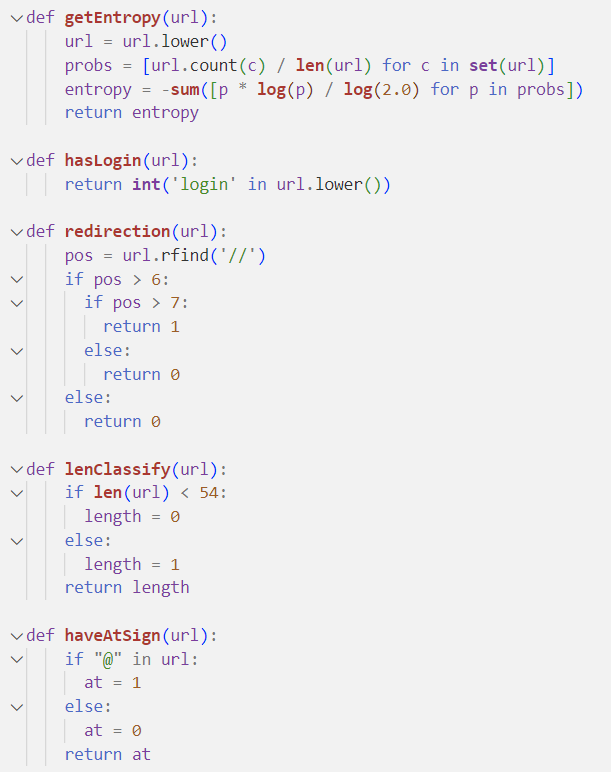
\includegraphics[width=0.45\textwidth]{featureExtraction_Code1.1.png}\label{fig:figure1}}
  \hfill
  {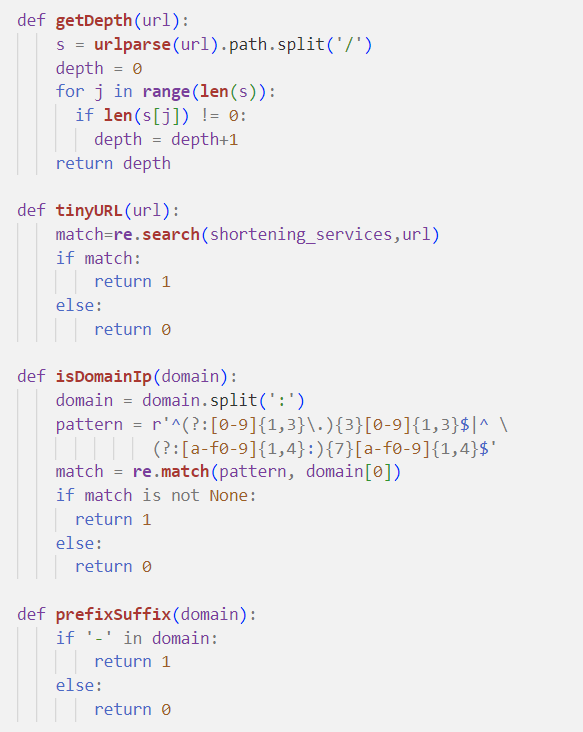
\includegraphics[width=0.450\textwidth]{featureExtraction_Code1.2.png}\label{fig:figure2}}
  \caption{Lexical Feature Extraction}
  \label{fig:bothfigures}
\end{figure}

\subsection{Numerical Features}
\par Numerical value-based features are features that represent quantitative or continuous values. These features can take on a wide range of numeric values and are often used in various machine learning algorithms and statistical analyses. 


\par Features of a URL are basically classified into - protocol, domain, path, query, fragment. The length of this each features and the count of the different special characters in that specific feature are extracted. The special characters like  ‘.’ ‘-’ ‘/’ ‘?’ ‘=’ ‘@’ ‘\&’ ‘!’ ‘\ ’ ‘{~}' ‘,’ ‘+’ ‘*’ ‘\#’ ‘\$’ ‘\%’ .
\par These features are :\\ 
{\footnotesize 
\begin{multicols}{3} % Set the number of columns you want
\begin{itemize}
\item url\_length
\item qty\_dot\_url
\item qty\_hyphen\_url
\item qty\_slash\_url
\item qty\_questionmark\_url
\item qty\_equal\_url
\item qty\_at\_url
\item qty\_and\_url
\item qty\_exclamation\_url
\item qty\_space\_url
\item qty\_tilde\_url
\item qty\_comma\_url
\item qty\_plus\_url
\item qty\_asterisk\_url
\item qty\_hashtag\_url
\item qty\_dollar\_url
\item qty\_percent\_url
\item domain\_length
\item qty\_dot\_domain
\item qty\_hyphen\_domain
\item path\_length
\item qty\_dot\_path
\item qty\_hyphen\_path
\item qty\_slash\_path
\item qty\_equal\_path
\item qty\_at\_path
\item qty\_and\_path
\item qty\_exclamation\_path
\item qty\_space\_path
\item qty\_tilde\_path
\item qty\_comma\_path
\item qty\_plus\_path
\item qty\_asterisk\_path
\item qty\_dollar\_path
\item qty\_percent\_path
\item query\_length
\item qty\_dot\_query
\item qty\_hyphen\_query
\item qty\_slash\_query
\item qty\_questionmark\_query
\item qty\_equal\_query
\item qty\_at\_query
\item qty\_and\_query
\item qty\_exclamation\_query
\item qty\_space\_query
\item qty\_tilde\_query
\item qty\_comma\_query
\item qty\_plus\_query
\item qty\_asterisk\_query
\item qty\_dollar\_query
\item qty\_percent\_query
\item fragment\_length
\item qty\_dot\_fragment
\item qty\_hyphen\_fragment
\item qty\_slash\_fragment
\item qty\_questionmark\_fragment
\item qty\_equal\_fragment
\item qty\_and\_fragment
\item qty\_exclamation\_fragment
\item qty\_space\_fragment
\item qty\_comma\_fragment
\item qty\_asterisk\_fragment
\item qty\_hashtag\_fragment
\item qty\_dollar\_fragment
\item qty\_percent\_fragment
\end{itemize}.
\end{multicols}
}
\par Finally, a total of 74 features are extracted in this project. After extracting both the Lexical and Numerical Features, they are saved to a new csv file for the Model Evaluation.
\begin{figure}[H]
\centerline{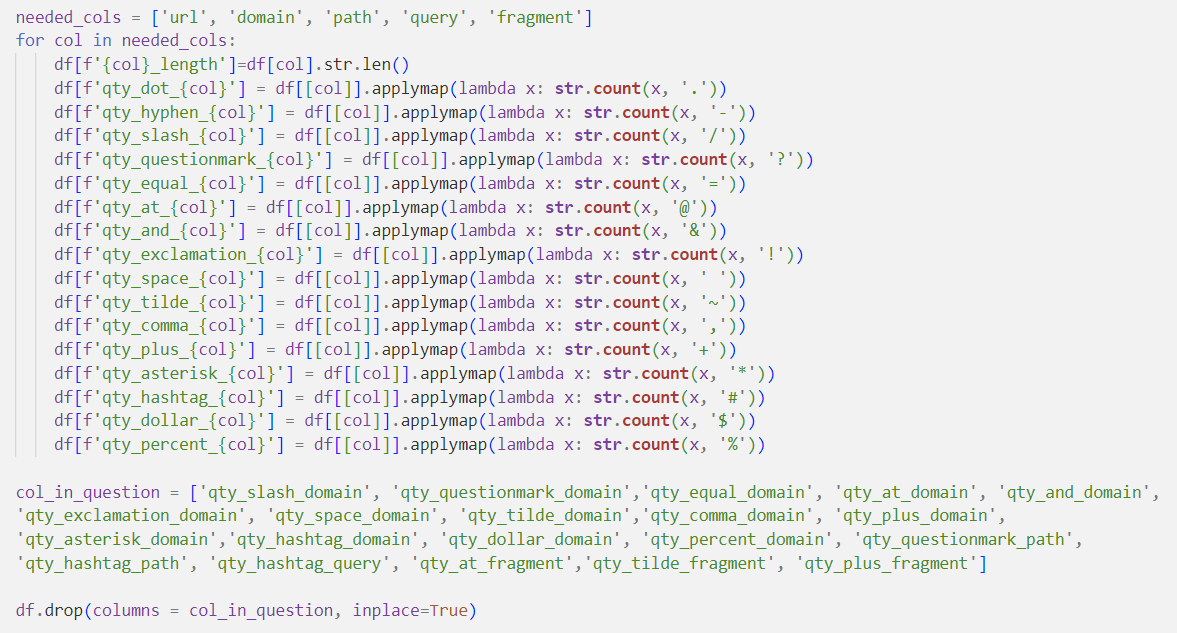
\includegraphics[scale=0.55]{featureExtraction_Code2.png}}
\caption{Numerical Feature Extraction}
\label{fig}
\end{figure}


\section{MODEL COMPARISON}
\subsection{Pycaret}
\par PyCaret is a Python library that provides an easy-to-use interface for training and comparing multiple machine learning models. It offers a variety of functions and tools to streamline the model development process and make it efficient. We use this library to compare the different machine learning models by using the extracted features and it will returns a table of model performance metrics sorted by  specified evaluation metrics - accuracy, AUC, recall, precision, F1, Kappa and MCC.

\par 15 different algorithms were compared and Logistic Regression(94.45\%) gave more accuracy among them. Thus, Logistic Regression model is used for testing and training the features. 
\begin{figure}[H]
\centerline{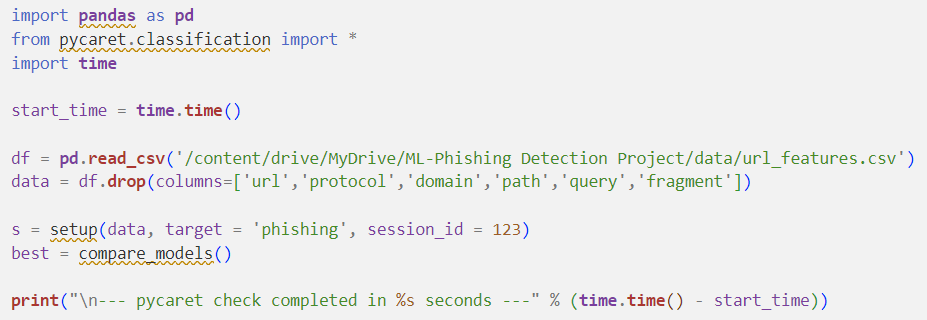
\includegraphics[scale=0.6]{pycaretCode.png}}
\caption{Pycaret Comparison}
\label{fig}
\end{figure}



\section{MODEL EVALUATION}
\par Model evaluation is a crucial step in machine learning to assess the performance and effectiveness of a trained model. It involves quantitatively measuring how well the model generalizes to new, unseen data and how accurately it predicts the target variable.Based on the model comparison, we evaluated the logistic regression(lr) model in this project.
\\
\par Evaluating a LR model includes the following steps:
\begin{itemize}
\item Spliting the dataset: Dividing dataset into training and testing sets, ensuring that both sets have a representative distribution of the target variable.
\item Training the LR model: Fiting the logistic regression model to the training data using a suitable library such as scikit-learn.
\item Make predictions: Use the trained model to predict the target variable for the test dataset.
\item Calculating evaluation metrics: Comparing the predicted values with the actual values from the test dataset and calculating the evaluation metrics such as accuracy, precision, recall, F1-score, AUC-ROC, and confusion matrix. Libraries like scikit-learn provide functions to calculate these metrics.
\end{itemize}

\begin{figure}[H]
\centerline{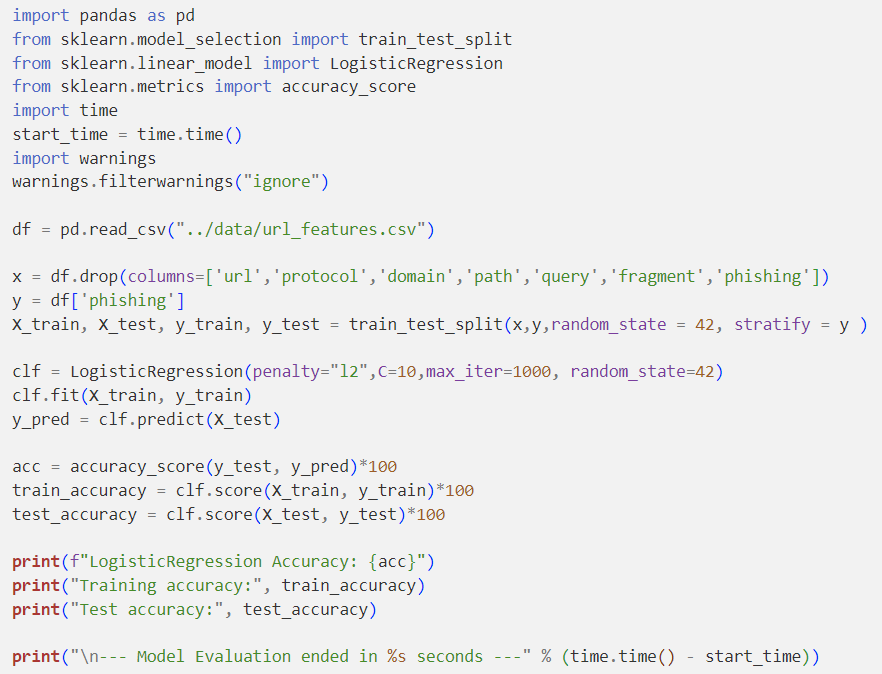
\includegraphics[scale=0.6]{modelEvaluation_Code.png}}
\caption{Model Evaluation}
\label{fig}
\end{figure}

\section{MODEL IMPLEMENTATION}
\par This phase involves deploying and integrating the trained machine learning model into a production environment where it can be used to make predictions on new, unseen data.This includes the following processes:
\begin{itemize}
\item Exporting the Model: Saving the trained model in a serialized format that can be easily loaded and used for predictions. We will be using python pickle module for exporting the trained lr model, which is a built-in module that provides a way to serialize and deserialize Python objects.
\item Model Integration: Integrating the model into the target application which is the WhalingGuard Web Appication where it will be used for predictions by API call.
\item Model Loading: Loading the serialized model into the implementation environment, making it ready for use. Again the pickle module is used to deserialize the model.
\item Input Data Feeding: Providing the new data, which is the URL to the model for prediction. This is done by passing the input data through a API call from the WhalingGuard User-Interface.
\item Feature Extraction: Extract the 74 different features from the input URL that where extracted during training phase. And saving that features to a new file for predicting.
\item Prediction Generation: Utilize the loaded model to generate predictions on the extracted features. Fiting the loaded model to the extracted features.  
\item Output Delivery: The prediction result is then passed to the API and the API then sends the results as a response to the frontend. The prediction results is also saved in csv file in the server, continously for each API calls.Then, at the user interface, the users can view the results whether the entered url is phishing or non-phishing.
\end{itemize}

\begin{figure}[H]
  \centering
  \subfloat[api.js]{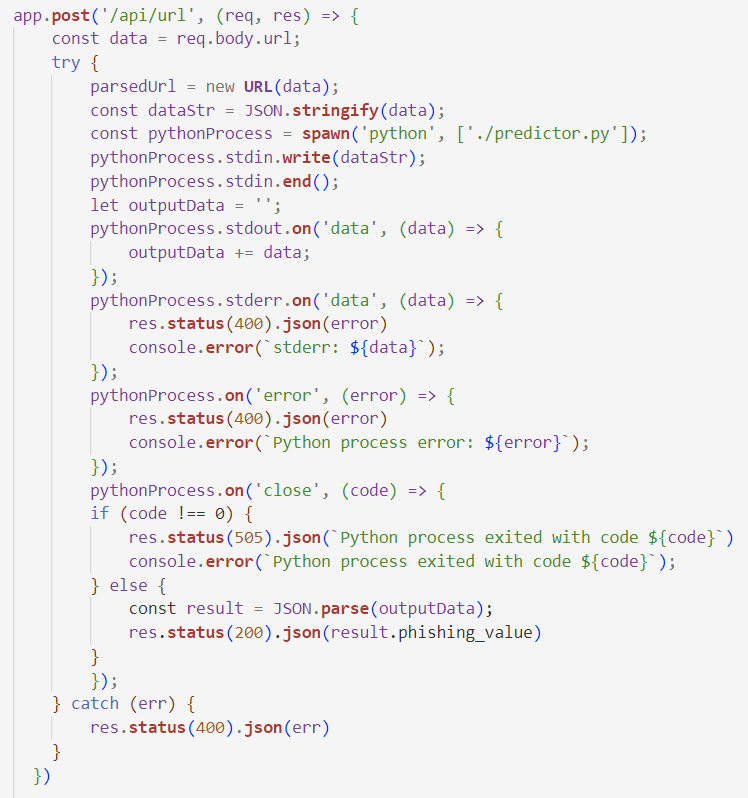
\includegraphics[width=0.47\textwidth]{apiCode.png}\label{fig:figure1}}
  \hfill
  \subfloat[predictor.py]{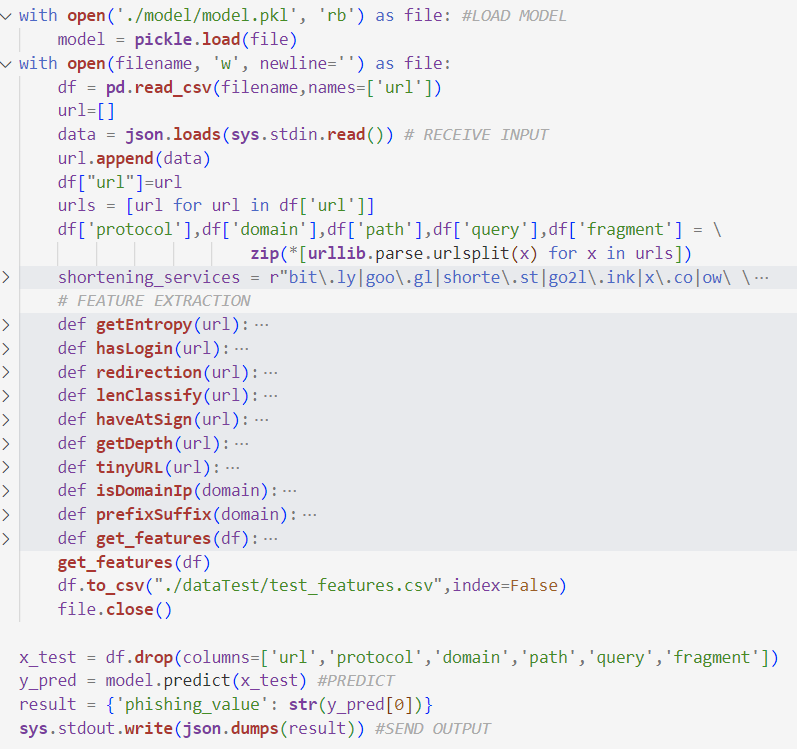
\includegraphics[width=0.47\textwidth]{predictorCode.png}\label{fig:figure2}}
  \label{fig:bothfigures}
\end{figure}
